%-----------------------------------------------------------------------------------------------------------------------------------------------%
%	The MIT License (MIT)
%
%	Copyright (c) 2015 Jan Küster
%
%	Permission is hereby granted, free of charge, to any person obtaining a copy
%	of this software and associated documentation files (the "Software"), to deal
%	in the Software without restriction, including without limitation the rights
%	to use, copy, modify, merge, publish, distribute, sublicense, and/or sell
%	copies of the Software, and to permit persons to whom the Software is
%	furnished to do so, subject to the following conditions:
%	
%	THE SOFTWARE IS PROVIDED "AS IS", WITHOUT WARRANTY OF ANY KIND, EXPRESS OR
%	IMPLIED, INCLUDING BUT NOT LIMITED TO THE WARRANTIES OF MERCHANTABILITY,
%	FITNESS FOR A PARTICULAR PURPOSE AND NONINFRINGEMENT. IN NO EVENT SHALL THE
%	AUTHORS OR COPYRIGHT HOLDERS BE LIABLE FOR ANY CLAIM, DAMAGES OR OTHER
%	LIABILITY, WHETHER IN AN ACTION OF CONTRACT, TORT OR OTHERWISE, ARISING FROM,
%	OUT OF OR IN CONNECTION WITH THE SOFTWARE OR THE USE OR OTHER DEALINGS IN
%	THE SOFTWARE.
%	
%
%-----------------------------------------------------------------------------------------------------------------------------------------------%


%============================================================================%
%
%	DOCUMENT DEFINITION
%
%============================================================================%

%we use article class because we want to fully customize the page and dont use a cv template
\documentclass[10pt,A4]{article}	


%----------------------------------------------------------------------------------------
%	ENCODING
%----------------------------------------------------------------------------------------

%we use utf8 since we want to build from any machine
\usepackage[utf8]{inputenc}		

%----------------------------------------------------------------------------------------
%	LOGIC
%----------------------------------------------------------------------------------------

% provides \isempty test
\usepackage{xifthen}

%----------------------------------------------------------------------------------------
%	FONT
%----------------------------------------------------------------------------------------

% some tex-live fonts - choose your own

%\usepackage[defaultsans]{droidsans}
%\usepackage[default]{comfortaa}
%\usepackage{cmbright}
%\usepackage[default]{raleway}
%\usepackage{fetamont}
\usepackage[default]{gillius}
%\usepackage[light,math]{iwona}
%\usepackage[thin]{roboto} 

% set font default
\renewcommand*\familydefault{\sfdefault} 	
\usepackage[T1]{fontenc}

% more font size definitions
\usepackage{moresize}		

\usepackage{fontawesome}

%----------------------------------------------------------------------------------------
%	PAGE LAYOUT  DEFINITIONS
%----------------------------------------------------------------------------------------

%debug page outer frames
%\usepackage{showframe}			


%define page styles using geometry
\usepackage[a4paper]{geometry}		

% for example, change the margins to 2 inches all round
\geometry{top=1cm, bottom=-.6cm, left=0.4cm, right=1cm} 	


%less space between header and content
\setlength{\headheight}{-5pt}		


%customize entries left, center and right
%\lhead{}
%\chead{ \small{Jan Küster  $\cdot$ Consultant and Software Engineer $\cdot$  Bremen, Germany  $\cdot$  \textcolor{sectcol}{\textbf{info@jankuester.com}}  $\cdot$ +49 176 313 *** **}}
%\rhead{}


%indentation is zero
\setlength{\parindent}{0mm}

%----------------------------------------------------------------------------------------
%	TABLE /ARRAY DEFINITIONS
%---------------------------------------------------------------------------------------- 

%for layouting tables
\usepackage{multicol}			
\usepackage{multirow}

%extended aligning of tabular cells
\usepackage{array}

\newcolumntype{x}[1]{%
>{\raggedleft\hspace{0pt}}p{#1}}%


%----------------------------------------------------------------------------------------
%	GRAPHICS DEFINITIONS
%---------------------------------------------------------------------------------------- 

%for header image
\usepackage{graphicx}

%for floating figures
\usepackage{wrapfig}
\usepackage{float}
%\floatstyle{boxed} 
%\restylefloat{figure}

%for drawing graphics		
\usepackage{tikz}				
\usetikzlibrary{shapes, backgrounds,mindmap, trees}


%----------------------------------------------------------------------------------------
%	Color DEFINITIONS
%---------------------------------------------------------------------------------------- 
\usepackage{transparent}
\usepackage{color}

%accent color
\definecolor{complcol}{RGB}{244,160,0}

%dark background color
\definecolor{bgcol}{RGB}{110,110,110}

%light background / accent color
\definecolor{softcol}{RGB}{219,68,55}

\definecolor{sectcol}{RGB}{66,133,244}

\definecolor{maya}{RGB}{124,185,232}

\definecolor{col1}{RGB}{66,133,244}
\definecolor{col2}{RGB}{219,68,55}
\definecolor{col3}{RGB}{244,160,0}
\definecolor{col4}{RGB}{15,157,88}
\definecolor{col5}{RGB}{251, 120, 56}

%Package for links, must be the last package used
\usepackage[hidelinks]{hyperref}

%============================================================================%
%
%
%	DEFINITIONS
%
%
%============================================================================%

% returns minipage width minus two times \fboxsep
% to keep padding included in width calculations
\newcommand{\mpwidth}{\linewidth-\fboxsep-\fboxsep}
	

%----------------------------------------------------------------------------------------
% 	ARROW GRAPHICS in Tikz
%----------------------------------------------------------------------------------------

% a six pointed arrow poiting to the left
\newcommand{\tzlarrow}{(0,0) -- (0.2,0) -- (0.3,0.2) -- (0.2,0.4) -- (0,0.4) -- (0.1,0.2) -- cycle;}	

% include the left arrow into a tikz picture
% param1: fill color
%
\newcommand{\larrow}[1]
{\begin{tikzpicture}[scale=0.58]
	 \filldraw[fill=#1!100,draw=#1!100!black]  \tzlarrow
 \end{tikzpicture}
}

% a six pointed arrow poiting to the right
\newcommand{\tzrarrow}{ (0,0.2) -- (0.1,0) -- (0.3,0) -- (0.2,0.2) -- (0.3,0.4) -- (0.1,0.4) -- cycle;}

% include the right arrow into a tikz picture
% param1: fill color
%
\newcommand{\rarrow}
{
\begin{tikzpicture}[scale=0.7]
	\filldraw[fill=softcol!100,draw=softcol!100!black] \tzrarrow
 \end{tikzpicture}
}

%----------------------------------------------------------------------------------------
%	custom sections
%----------------------------------------------------------------------------------------

% create a coloured box with arrow and title as cv section headline
% param 1: section title
%
\newcommand{\cvsection}[1]
{
\colorbox{sectcol}{\mystrut \makebox[1\mpwidth][l]{
\larrow{softcol} \hspace{-8pt} \larrow{softcol} \hspace{-8pt} \larrow{softcol} \textbf{\textcolor{white}{\uppercase{#1}}}\hspace{4pt}
}}\\
}


\newcommand{\cvskill}[3] {
	\begin{tabular*}{1\mpwidth}{p{0.75\mpwidth}  r}
		\textcolor{white}{\textbf{#1}} & \textcolor{white}{\textbf{#2}}\\
	\end{tabular*}%
	\hspace{1pt}
	\begin{tikzpicture}[scale=1,rounded corners=2pt,very thin]
	\fill [white] (0,0) rectangle (1\mpwidth, 0.15);
	\fill [col4] (0,0) rectangle (#3\mpwidth, 0.15);
	\end{tikzpicture}%
}

% create a coloured arrow with title as cv meta section section
% param 1: meta section title
%
\newenvironment{metasection}[1] {
	\vspace{6pt}
	\begin{center}
		\textcolor{white}{\large{\uppercase{#1}}}\\
	\normalsize
	\parbox{0.7\mpwidth}{\textcolor{white}	\hrule}
}{\end{center}}

%----------------------------------------------------------------------------------------
%	 CV EVENT
%----------------------------------------------------------------------------------------

% creates a stretched box as cv entry headline followed by two paragraphs about 
% the work you did
% param 1:	event time i.e. 2014 or 2011-2014 etc.
% param 2:	event name (what did you do?)
% param 3:	institution (where did you work / study)
% param 4:	what was your position
% param 5:	some words about your contributions
%
\newcommand{\cvevent}[5]
{
\vspace{8pt}
	\begin{tabular*}{1\mpwidth}{p{0.55\mpwidth}  x{0.42\mpwidth}}
 	\textcolor{black}{\textbf{#2}} & \textcolor{softcol}{#3}, \textcolor{bgcol}{\textbf{#1}} 

	\end{tabular*}
\vspace{-12pt}
\textcolor{softcol}{\hrule}
\vspace{6pt}
	\begin{tabular*}{0.5\mpwidth}{p{\mpwidth}}
\larrow{softcol}  #4\\[3pt]
\larrow{softcol}  #5\\[6pt]
	\end{tabular*}

}

% creates a stretched box as 
\newcommand{\cveventmeta}[2]
{
	\mbox{\mystrut \hspace{87pt}\textit{#1}}\\
	#2
}

%----------------------------------------------------------------------------------------
% CUSTOM STRUT FOR EMPTY BOXES
%----------------------------------------- -----------------------------------------------
\newcommand{\mystrut}{\rule[-.3\baselineskip]{0pt}{\baselineskip}}

%----------------------------------------------------------------------------------------
% CUSTOM LOREM IPSUM
%----------------------------------------------------------------------------------------
\newcommand{\lorem}
{Lorem ipsum dolor sit amet, consectetur adipiscing elit. Donec a diam lectus.}


% use to vertically center content
% credits to: http://tex.stackexchange.com/questions/7219/how-to-vertically-center-two-images-next-to-each-other
\newcommand{\vcenteredinclude}[1]{\begingroup
\setbox0=\hbox{\includegraphics{#1}}%
\parbox{\wd0}{\box0}\endgroup}

% use to vertically center content
% credits to: http://tex.stackexchange.com/questions/7219/how-to-vertically-center-two-images-next-to-each-other
\newcommand*{\vcenteredhbox}[1]{\begingroup
\setbox0=\hbox{#1}\parbox{\wd0}{\box0}\endgroup}

%----------------------------------------------------------------------------------------
%	ICON-SET EMBEDDING
%---------------------------------------------------------------------------------------- 

% at this point we simplify our icon-embedding by simply referring to a set of png images.
% if you find a good way of including svg without conflicting with other packages you can
% replace this part
\newcommand{\icon}[3]{\makebox(#2, #2){\textcolor{#3}{\csname fa#1\endcsname}}}	%icon shortcut
\newcommand{\icontext}[4]{ 						%icon with text shortcut
	\vcenteredhbox{\icon{#1}{#2}{#4}} \vcenteredhbox{\textcolor{#4}{#3}}
}
\newcommand{\iconhref}[5]{ 						%icon with website url
    \vcenteredhbox{\icon{#1}{#2}{#5}} \href{#4}{\textcolor{#5}{#3}}
}

\newcommand{\iconemail}[5]{ 						%icon with email link
    \vcenteredhbox{\icon{#1}{#2}{#5}} \href{mailto:#4}{\textcolor{#5}{#3}}
}

%----------------------------------------------------------------------------------------
% 	PIE CHART
%----------------------------------------------------------------------------------------
%-----------------------------------------------------------------------------------------------------------------------------------------------%
%	The MIT License (MIT)
%
%	Copyright (c) 2016 Jan Küster
%
%	Permission is hereby granted, free of charge, to any person obtaining a copy
%	of this software and associated documentation files (the "Software"), to deal
%	in the Software without restriction, including without limitation the rights
%	to use, copy, modify, merge, publish, distribute, sublicense, and/or sell
%	copies of the Software, and to permit persons to whom the Software is
%	furnished to do so, subject to the following conditions:
%	
%	THE SOFTWARE IS PROVIDED "AS IS", WITHOUT WARRANTY OF ANY KIND, EXPRESS OR
%	IMPLIED, INCLUDING BUT NOT LIMITED TO THE WARRANTIES OF MERCHANTABILITY,
%	FITNESS FOR A PARTICULAR PURPOSE AND NONINFRINGEMENT. IN NO EVENT SHALL THE
%	AUTHORS OR COPYRIGHT HOLDERS BE LIABLE FOR ANY CLAIM, DAMAGES OR OTHER
%	LIABILITY, WHETHER IN AN ACTION OF CONTRACT, TORT OR OTHERWISE, ARISING FROM,
%	OUT OF OR IN CONNECTION WITH THE SOFTWARE OR THE USE OR OTHER DEALINGS IN
%	THE SOFTWARE.
%
%-----------------------------------------------------------------------------------------------------------------------------------------------%

%counters for chart loop
\newcounter{a}
\newcounter{b}
\newcounter{c}

% draw a slice for a chart
% param 1: Circle form - 90 = quarter, 180 = half, 360 = full
% param 2: scale default=1 (scales only chart, not label text)
% param 3: border color
% param 4: label text color
% param 5: label bg color
% param 6:
\newenvironment{piechart}[5] {

	% draw a slice for a chart
	% param 1: value x of 100
	% param 2: label text
	% param 3: fill color
	% param 4:
	% param 5:
	% param 6:
	\newcommand{\slice}[3] {

		\setcounter{a}{\value{b}}
		\addtocounter{b}{##1}

		%set from angle point
		\pgfmathparse{\thea/100*#1}
	  	\let\pointa\pgfmathresult

		%set toanglepoint
		\pgfmathparse{\theb/100*#1}
	  	\let\pointb\pgfmathresult

		%set midangle
	 	\pgfmathparse{0.5*\pointa+0.5*\pointb}
	  	\let\midangle\pgfmathresult
		
		% draw the slice
	  	\filldraw[fill=##3!100,draw=#3!100, line width=2pt ] (0,0) -- (\pointa:#2) arc (\pointa:\pointb:#2) -- cycle;

	  	% draw label
	  	\node[label=\midangle:\colorbox{#5}{\textcolor{#4}{##2}}] at (\midangle:#2) {};

		\filldraw[fill=#3,draw=none] (0,0) circle (#2/2);
	}

	% execute commands
	\setcounter{a}{0}
	\setcounter{b}{0}
	\begin{tikzpicture}
}
{\end{tikzpicture}}

%============================================================================%
%
%
%
%	DOCUMENT CONTENT: ENGLISH
%
%
%
%============================================================================%
\begin{document}
\fcolorbox{white}{white}{\begin{minipage}[c][0.96\textheight][t]{0.7\linewidth}


%---------------------------------------------------------------------------------------
%	TITLE HEADLINE
%----------------------------------------------------------------------------------------
\vspace{-3pt}
% use this for multiple words like working titles etc.
%\hspace{-0.25\linewidth}\colorbox{bgcol}{\makebox[1.5\linewidth][c]{\hspace{46pt}\HUGE{\textcolor{white}{\uppercase{M.Sc. Jan Küster}} } \textcolor{sectcol}{\rule[-1mm]{1mm}{0.9cm}} \parbox[b]{5cm}{   \large{ \textcolor{white}{{IT Consultant}}}\\
% \large{ \textcolor{white}{{JS Fullstack Engineer}}}}
%}}
% use this for single words, e.g. CV or RESUME etc.
\colorbox{bgcol}{\makebox[\mpwidth][c]{\HUGE{\textcolor{white}{\uppercase{Alan Matzumiya}} } \textcolor{softcol}{\rule[-1mm]{1mm}{0.9cm}} \HUGE{\textcolor{white}{\uppercase{English}} } }}

%----------------------------------------------------------------------------------------
%	HEADER IMAGE
%----------------------------------------------------------------------------------------


%\hspace{-1.6cm}
%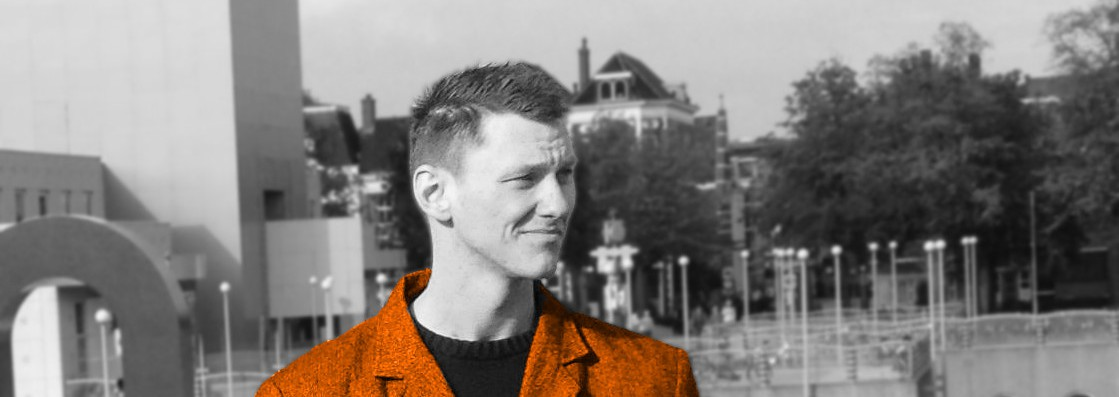
\includegraphics[trim= 0 250 0 270,clip,width=1\linewidth+3.1cm]{myfoto.jpg}	%trimming relative to image size!
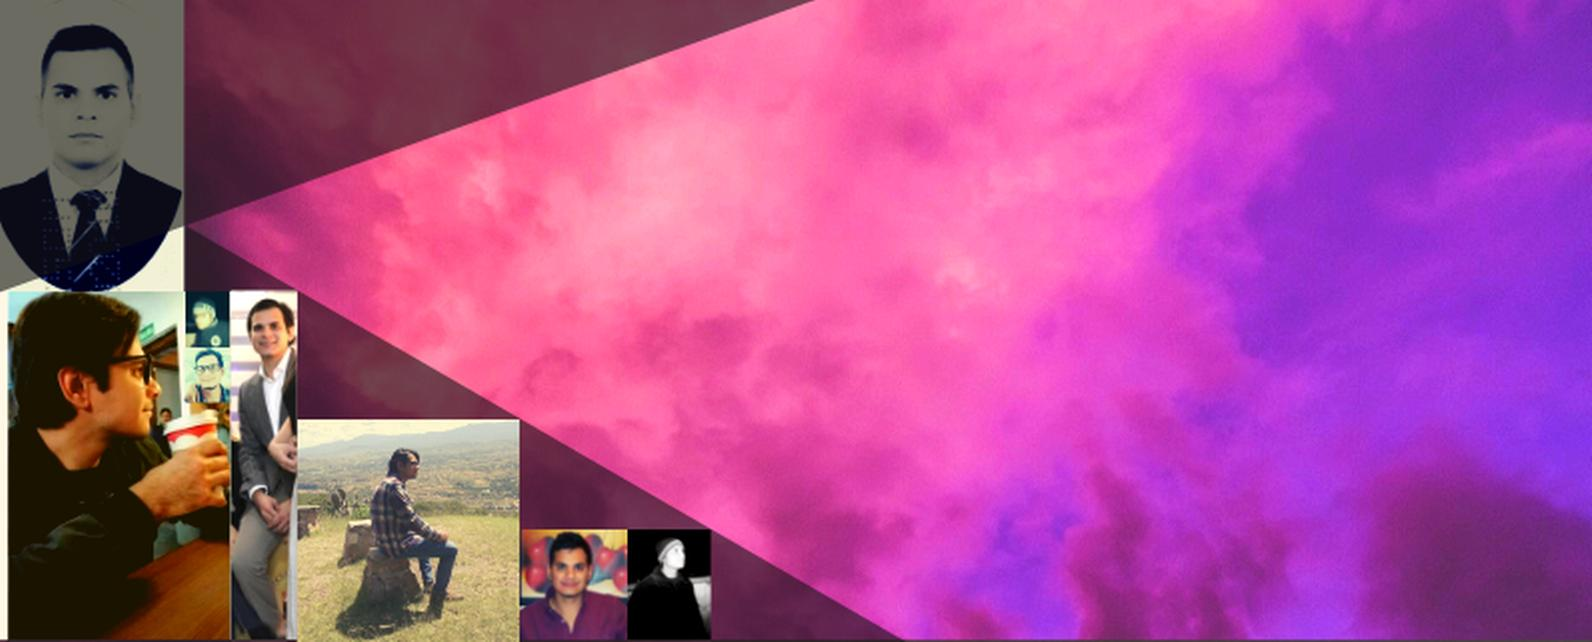
\includegraphics[width=0.9995\linewidth]{banner.jpg}	%trimming relative to image size

%---------------------------------------------------------------------------------------
%	SUMMARY
%----------------------------------------------------------------------------------------
\transparent{0.85}%
\vspace{-127pt}
\hspace{0.32\linewidth}
\colorbox{bgcol}{
	\parbox{0.60\linewidth}{\vspace{-1.15mm}\hspace{-0.028\linewidth}\colorbox{softcol}{\parbox{1.028\linewidth}{\textcolor{white}{\hspace{0.22\linewidth}Alan Daniel Matzumiya Zazueta}}}
		\vspace{-4.5mm}
		\begin{center}
		\larrow{softcol}\larrow{softcol} \textcolor{white}{I'm Chemical Engineer and M.Sc. Mathematics.\\I'm Also Python Full Stack Focused on Data Analysis and Software / Web Development}
		\end{center}
	}
}
\vspace{60pt}
\transparent{1}%
%============================================================================%
%
%	CV SECTIONS AND EVENTS (MAIN CONTENT)
%
%============================================================================%

%---------------------------------------------------------------------------------------
%	STATUS
%----------------------------------------------------------------------------------------
\cvsection{About Me}

\colorbox{sectcol}{
	\parbox{0.969\linewidth}{
	\parbox{0.45\linewidth}{
	\begin{itemize}
		\item[\larrow{softcol}] \textcolor{white}{\textbf{Age: 28 years}}
		\item[\larrow{softcol}] \textcolor{white}{\textbf{Birthday: 14 Sept 1992}}
		\item[\larrow{softcol}] \textcolor{white}{\textbf{Hometown: Guaymas, Son}}
		\item[\larrow{softcol}] \textcolor{white}{\textbf{Residency: Hermosillo, Son}}
	\end{itemize}
	}
	\parbox{0.4\linewidth}{
	\begin{itemize}
		\item[\larrow{softcol}] \textcolor{white}{\textbf{Native Language: Spanish}}  
		\item[\larrow{softcol}]	\cvskill{Speak English} {80 \%} {0.8}
		\item[\larrow{softcol}]	\cvskill{Write English} {90 \%} {0.9}
	\end{itemize}
	}
	}
}
\vspace{5pt}

%---------------------------------------------------------------------------------------
%	EXPERIENCE
%----------------------------------------------------------------------------------------
\cvsection{Experience}

%
\cvevent{May-Aug 2015}{Professional Practices}{CFE, Hermosillo}{Environmental audit assistant in plant}{Project proposal developed to modify water treatment plant}

%\textcolor{softcol}{\hrule}

%
\cvevent{June-Sept 2018}{Scientific Researching}{UNAM, Oaxaca}{Studies about numerical methods to solve stochastic partial differential equations}{The article publication can be consulted at the following button: \hspace{2mm} \href{https://www.researchgate.net/publication/334330862_INITIAL_CONDITIONS_CONTINUITY_OF_A_NUMERICAL_APPROXIMATION_FOR_KOLMOGOROV_EQUATIONS/}{\colorbox{bgcol}{\colorbox{white}{\hspace{3mm}\textcolor{bgcol}{\textbf{Get Info}} \hspace{1.5mm} \icon{Info}{8}{bgcol}\hspace{3mm}}}}}

%\textcolor{softcol}{\hrule}

%
\cvevent{2017 - 2019}{Programming Workshops}{Unison, Hermosillo}{Programming class teacher developed in Jupyter Notebook using Python language and oriented to engineering students}{The class material can be consulted at the following button: \hspace{8mm} \href{https://circuitalminds.github.io/pyfullstack/}{\colorbox{bgcol}{\colorbox{white}{\hspace{1mm}{\textcolor{bgcol}{\textbf{Notebooks}} \hspace{1.5mm} \icon{Github}{8}{bgcol}\hspace{1mm}}}}}}

%\textcolor{softcol}{\hrule}

%
\cvevent{2019 - Now}{Programming Projects}{GitHub}{
	Python package to solving PDE's including its stochastic versions \hspace{0.25mm} \href{https://www.github.com/alanmatzumiya/Paper/}{\colorbox{bgcol}{\colorbox{white}{\hspace{0mm} \textcolor{bgcol}{\textbf{Repository}} \hspace{1.5mm} \icon{Github}{8}{bgcol} \hspace{0mm}}}}
	\vspace{1mm}}
	{
	Python Package to build spectral numerical methods \hspace{18mm} \href{https://www.github.com/alanmatzumiya/pySpectralPDE}{\colorbox{bgcol}{\colorbox{white}{\hspace{1.060mm}\textcolor{bgcol}{\textbf{Repository}} \hspace{1.5mm} \icon{Github}{8}{bgcol}\hspace{1.060mm}}}}
	\vspace{1mm}
}

\vspace{5pt}
%---------------------------------------------------------------------------------------
%	EDUCATION SECTION
%--------------------------------------------------------------------------------------
\cvsection{Education}

\cvevent{2017 - 2019}{
	Master Degree in Mathematical Sciences}{Unison, Hermosillo}{Thesis: Numerical Solutions to the Stochastic and Deterministic Burgers Equation Using Spectral Methods
	}
	{
	Click on the following button to download thesis file: \hspace{18mm} \href{https://github.com/alanmatzumiya/pySpectralPDE/raw/master/docs/Thesis.pdf}{\colorbox{bgcol}{\colorbox{white}{\textcolor{bgcol}{\hspace{3mm}\textbf{Get PDF}} \hspace{1.5mm} \icon{Download}{8}{bgcol}\hspace{3mm}}}}
}

%\textcolor{sectcol}{\hrule}

%
\cvevent{2011 - 2016}{Bachelor in Chemical Engineering}{Unison, Hermosillo}{
	Thesis: Caracterizaci\'on y evaluaci\'on de las propiedades bioactivas de una mezcla de biocomp\'ositos de hidroxiapatita/$\beta$-wollastonita
	}
	{
	Click on the following button to download thesis file: \hspace{18mm} \href{http://www.repositorioinstitucional.uson.mx/handle/unison/1840}{\colorbox{bgcol}{\colorbox{white}{\textcolor{bgcol}{\hspace{3mm}\textbf{Get PDF}} \hspace{1.5mm} \icon{Download}{8}{bgcol}\hspace{3mm}}}}
}


\end{minipage}}%
\fcolorbox{white}{sectcol}{\begin{minipage}[c][0.96\textheight][t]{0.33\linewidth}


\begin{metasection}{Contact}

	\icontext{MapMarker}{12}{Hermosillo, Sonora}{white}\\[6pt]
	
	\iconhref{Whatsapp}{12}{\textbf{+52 662 364 8525}}{https://api.whatsapp.com/send?phone=5216623648525\&text=Hola\%20Alan,\%20Buen\%20D\%C3\%ADa.}{white}\\[6pt]
	
	\iconemail{Send}{12}{\textbf{alan.matzumiya@gmail.com}}{alan.matzumiya@gmail.com}{white}\\[6pt]
	
	\iconhref{Link}{12}{\textbf{alanmatzumiya.github.io}}{https://alanmatzumiya.github.io/}{white}\\[6pt]
	
	\iconhref{Link}{12}{\textbf{Circuital Minds}}{https://circuitalminds.github.io/}{white}\\[6pt]
	
	\LARGE{
	\href{https://www.github.com/alanmatzumiya/}{\icon{Github}{12}{white}}
	\hspace{1mm}
	\href{https://www.linkedin.com/in/alanmatzumiya/}{\icon{LinkedinSquare}{12}{white}}
	\hspace{1mm} 
	\href{https://www.facebook.com/alanmatzumiya/}{\icon{FacebookOfficial}{12}{white}}
	\hspace{1mm} 
	\href{https://www.instagram.com/alanmatzumiya/}{\icon{Instagram}{12}{white}}
	\hspace{1mm} 
	\href{https://www.pinterest.com/alanmatzumiya/}{\icon{Pinterest}{12}{white}}}\\[6pt]
	
\end{metasection}
		
%----------------------------------------------------------------------------------------
%	META SECTION
%----------------------------------------------------------------------------------------

\begin{metasection}{Skills}

	\vspace{2pt}
	
	\icontext{Tasks}{12}{Software / Web Development}{white}\\
	\icon{Star}{12}{complcol}\icon{Star}{12}{complcol}\icon{Star}{12}{complcol}\icon{Star}{12}{complcol}\icon{Star}{12}{complcol}\icon{Star}{12}{complcol}\icon{Star}{12}{complcol}\icon{Star}{12}{complcol}\icon{Star}{12}{white}\icon{Star}{12}{white}\\[6pt]
	
	\icontext{BarChart}{12}{Numerical Algorithms / Data Analysis}{white}\\
	\icon{Star}{12}{complcol}\icon{Star}{12}{complcol}\icon{Star}{12}{complcol}\icon{Star}{12}{complcol}\icon{Star}{12}{complcol}\icon{Star}{12}{complcol}\icon{Star}{12}{complcol}\icon{Star}{12}{complcol}\icon{Star}{12}{complcol}\icon{Star}{12}{complcol}\\[6pt]
	
	\vspace{6pt}
	
	\cvskill{\icontext{Code}{12}{Python / JavaScript}{white}} {4+ yrs} {1} \\[6pt]
	\cvskill{\icontext{Code}{12}{Visual Basic / PHP}{white}} {5+ yrs} {0.85} \\[6pt]
	\cvskill{\icontext{Code}{12}{C++ / Fortran}{white}} {5+ yrs} {1} \\[6pt]
	\cvskill{\icontext{AreaChart}{12}{R / Matlab}{white}} {4+ yrs} {0.90} \\[6pt]
	\cvskill{\icontext{Code}{12}{HTML / CSS / Markdown}{white}} {5+ yrs} {0.95} \\[6pt]
	\cvskill{\icontext{Database}{12}{MySQL / MariaDB}{white}} {3+ yrs} {0.90} \\[6pt]
	
\end{metasection}

\begin{metasection}{Technologies}

\textcolor{white}{\LARGE{\icon{Linux}{24}{white} \icon{Windows}{24}{white}} \icon{Android}{24}{white}}\\[6pt]

\icontext{GithubAlt}{12}{Git /}{white}  \icontext{Check}{12}{Selenium /}{white} 
\icontext{Exchange}{12}{Docker}{white} \\[6pt]

\icontext{Server}{12}{Django / Flask / Dash}{white} \\[6pt]

\icontext{Google}{12}{Google Analytics}{white} \icontext{Android}{12}{Android Studio}{white} \\[6pt]

\icontext{Code}{12}{PyCharm / Visual Studio}{white}\\[6pt]

\icontext{LineChart}{12}{Jupyter Notebook / RStudio}{white}

\end{metasection}

\begin{metasection}{Activities}

\vspace{6pt}	

\begin{piechart}{360}{-2}{maya}{maya}{white}
	\slice{30}{\LARGE{\icon{Desktop}{2}{white}}}{col1}
	\slice{30}{\LARGE{\icon{Bicycle}{8}{white}}}{col2}
	\slice{15}{\LARGE{\icon{Headphones}{0}{white}}}{col3}
	\slice{15}{\LARGE{\icon{Gamepad}{-4}{white}}}{col4}
	\slice{10}{\LARGE{\icon{Beer}{2}{sectcol}}}{white}
\end{piechart}

\end{metasection}

\end{minipage}}
%-------------------------------------------------------------------------------------------------
%	ARTIFICIAL FOOTER (fancy footer cannot exceed linewidth) 
%--------------------------------------------------------------------------------------------------

\vspace{1mm}
\null
\vspace*{\fill}
\hspace{-0.25\linewidth}\colorbox{bgcol}{
	\makebox[1.45\linewidth][c]{
		\mystrut \small \textcolor{white}{
			Coypright 2020 Alan Matzumiya}
	}
}

\newpage
%---------------------------------------------------------------------------------------
%	PROJECTS
%----------------------------------------------------------------------------------------
\parbox{1\linewidth}{
	\cvsection{Projects}
	
\includegraphics[width=1.0\linewidth]{screen_CircuitalMinds_git.png}
}
\parbox{1\linewidth}{	
	\cvevent{}
	{
		Website Built by Jekyll Themes
	}
	{ 
		\parbox{1\linewidth}{
			{\href{https://circuitalminds.github.io/}
				{
					{\colorbox{gray}{\hspace{7mm}\textcolor{white}{\textbf{CircuitalMinds}} \hspace{1.5mm} \icon{Github}{8}{white}\hspace{7mm}}}}
			}
		}
	}
	{
		Organization website called CircuitalMinds
	}
	{
		Contains its own blog and an extended course to learn Python programming
	}
}
\parbox{1\linewidth}{
	\cvevent{
	}
	{
		Set of applications using flask
	}
	{ 
		\parbox{1\linewidth}{
			{\href{https://circuitalminds.herokuapp.com/fractalmetric}	
				{
					{\colorbox{gray}{\hspace{7.5mm}\textcolor{white}{\textbf{FractalMetric}} \hspace{1.5mm} \icon{Github}{8}{white}\hspace{7.5mm}}}}
			}	
		}
	}
	{
		This application contains the most common snippets and wrappers to build large web pages, giving an advantage due to its ease
of use.
	}
	{
		Its main objective is to scale to manage and maintain the resources used by CircuitalMinds
	}
}
\parbox{1\linewidth}{
	\cvevent{
	}
	{
		Container-server for Jupyter Notebooks
	}
	{ \parbox{1\linewidth}{
			{\href{https://nbsanalysis.herokuapp.com/notebooks/}	
				{
					{\colorbox{gray}{\hspace{3mm}\textcolor{white}{\textbf{Jupyter Notebooks}} \hspace{1.5mm} \icon{Github}{8}{white}\hspace{3mm}}}}
			}
		}
	}
	{
		A container of notebooks that are prepared using Docker Hub with the help of a Pipeline, which are part of the resources of pyFullStack
	}
	{
		With an automated process, the production of an application served in Heroku is carried out using Flask and being able to use the
notebooks in Jupyter.
	}
}
\parbox{1\linewidth}{
	\cvevent{
	}
	{
		My home server
	}
	{ 
		\parbox{1\linewidth}{
			{\href{https://matsuhub.herokuapp.com/}
				{
					{\colorbox{gray}{\hspace{9.5mm}\textcolor{white}{\textbf{MatsuHub}} \hspace{1.5mm} \icon{Github}{8}{white}\hspace{9.5mm}}}}
			}
		}
	}
	{
		This development is simply a product of FractalMetric, which is used locally to access my files.
	}
	{
		It is also useful to listen to music downloaded through a wrapper to obtain YouTube videos
	}
}
\vspace{10pt}
\colorbox{gray}{
	\parbox{1.0\linewidth}{
		
		\colorbox{bgcol}{
			\parbox{0.98\linewidth}{
				\cvsection{Presentation}
				
				\parbox{1\linewidth}{
					
					\textcolor{white}{ \colorbox{sectcol}{
							By: Alan Matzumiya
						}
						\vspace{5pt}
					}	
					
				}
				\parbox{1\linewidth}{
					\textcolor{white}{
						The academic level that I have currently achieved characterizes me with a multidisciplinary training. However, it has not been my
only resource to develop skills and knowledge, since I constantly reinforce a self-taught discipline that is used to obtain a broad
vision in relation to my areas of personal interest.
						\\\\
						The knowledge that I consider to highlight is the use of mathematics in different contexts such as its applications in physics and
statistics; including its theoretical and practical understanding complementing it with the use of programming languages that were
mentioned above, since I take advantage of having a fairly broad knowledge about them.
						\\\\
						However, in relation to my programming knowledge, my goal is to have a knowledge of the Python language at a professional level, and I currently have a good advantage considering this language as my greatest programming resource that allows me
to go deeply enough in various related areas.
						\\\\
						You are free to read my projects considered for this document, and in case you have an interest in any that could be useful to you, with all the confidence you can count on my disposal and with pleasure provide the required information. Furthermore, if
you have the impression that I can be considered part of your team, you can certainly count on me.
						\\\\
						\textcolor{col2}{Important:} I consider myself a good element for having the ability to understand details, order and document in the best
possible way for future readers; As a mathematician and researcher, this dynamic is a fundamental practice that does not generate
retrogression.
						\\\\
						\vspace{5pt}
					}
				}
			}	
		}
	}
}

\null
\vspace*{\fill}
\hspace{-0.25\linewidth}\colorbox{bgcol}{\makebox[1.45\linewidth][c]{\mystrut \small \textcolor{white}{Coypright 2020 Alan Matzumiya}}}

\vspace{1mm}
\newpage
%============================================================================%
%
%
%
%	DOCUMENT CONTENT: SPANISH
%
%
%
%============================================================================%
\fcolorbox{white}{white}{\begin{minipage}[c][0.96\textheight][t]{0.7\linewidth}
		%---------------------------------------------------------------------------------------
		%	TITLE HEADLINE
		%----------------------------------------------------------------------------------------
		\vspace{-3pt}
		% use this for multiple words like working titles etc.
		%\hspace{-0.25\linewidth}\colorbox{bgcol}{\makebox[1.5\linewidth][c]{\hspace{46pt}\HUGE{\textcolor{white}{\uppercase{M.Sc. Jan Küster}} } \textcolor{sectcol}{\rule[-1mm]{1mm}{0.9cm}} \parbox[b]{5cm}{   \large{ \textcolor{white}{{IT Consultant}}}\\
		% \large{ \textcolor{white}{{JS Fullstack Engineer}}}}
		%}}
		% use this for single words, e.g. CV or RESUME etc.
		\colorbox{bgcol}{\makebox[\mpwidth][c]{\HUGE{\textcolor{white}{\uppercase{Alan Matzumiya}} } \textcolor{softcol}{\rule[-1mm]{1mm}{0.9cm}} \HUGE{\textcolor{white}{\uppercase{Español}} } }}
		
		%----------------------------------------------------------------------------------------
		%	HEADER IMAGE
		%----------------------------------------------------------------------------------------
		
		
		%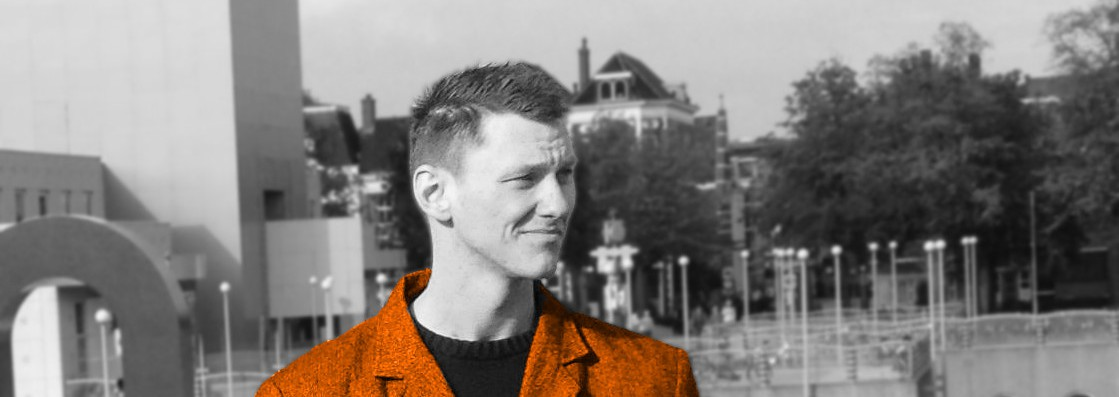
\includegraphics[trim= 0 250 0 270,clip,width=1\linewidth+3.1cm]{myfoto.jpg}	%trimming relative to image size!
		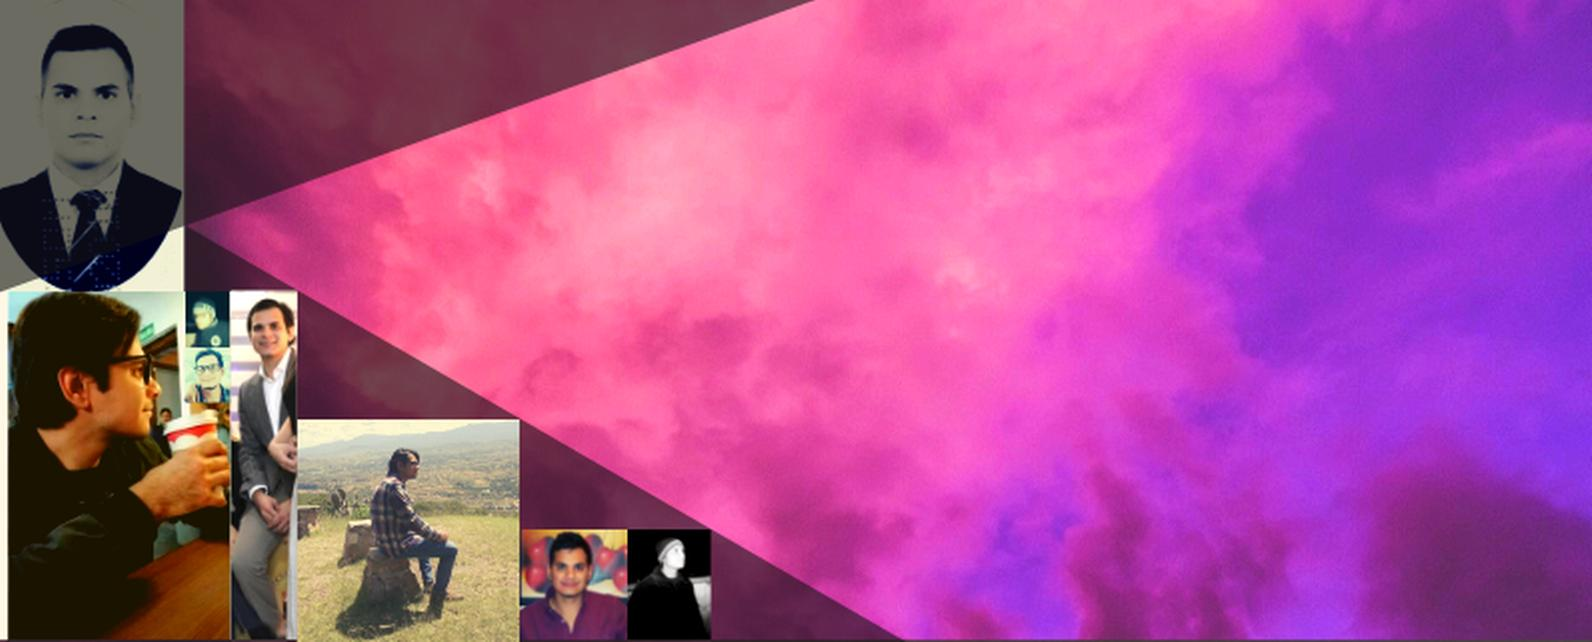
\includegraphics[width=0.9995\linewidth]{banner.jpg}	%trimming relative to image size
		
		%---------------------------------------------------------------------------------------
		%	SUMMARY
		%----------------------------------------------------------------------------------------
		\transparent{0.85}%
		\vspace{-127pt}
		\hspace{0.32\linewidth}
		\colorbox{bgcol}{
			\parbox{0.60\linewidth}{\vspace{-1.15mm}\hspace{-2.28mm}\colorbox{softcol}{\parbox{1.028\linewidth}{\textcolor{white}{\hspace{0.22\linewidth}Alan Daniel Matzumiya Zazueta}}}
				\vspace{-4.5mm}
				\transparent{1}%
				\begin{center}
					\larrow{softcol}\larrow{softcol} \textcolor{white}{Soy Ingeniero Qu\'imico y Maestro en Ciencias Matem\'aticas. Adem\'as, Soy Python Full Stack Enfocado en An\'alisis de Datos y Desarrollo de Software / Web}
				\end{center}
			}
		}
		\vspace{59.5pt}
		\transparent{1}%
		%============================================================================%
		%
		%	CV SECTIONS AND EVENTS (MAIN CONTENT)
		%
		%============================================================================%
		
		%---------------------------------------------------------------------------------------
		%	STATUS
		%----------------------------------------------------------------------------------------
		\cvsection{Acerca de Mi}
		
		\colorbox{sectcol}{
			\parbox{0.969\linewidth}{
				\parbox{0.45\linewidth}{
					\begin{itemize}
						\item[\larrow{softcol}] \textcolor{white}{\textbf{Edad: 28 años}}
						\item[\larrow{softcol}] \textcolor{white}{\textbf{Nacimiento: 14 Sept 1992}}
						\item[\larrow{softcol}] \textcolor{white}{\textbf{Lugar de Origen: Guaymas, Son}}
						\item[\larrow{softcol}] \textcolor{white}{\textbf{Residencia: Hermosillo, Son}}
					\end{itemize}
				}
				\parbox{0.4\linewidth}{
					\begin{itemize}
						\item[\larrow{softcol}] \textcolor{white}{\textbf{Lenguaje Nativo: Español}}  
						\item[\larrow{softcol}]	\cvskill{Hablar Ingl\'es} {80 \%} {0.8}
						\item[\larrow{softcol}]	\cvskill{Escribir Ingl\'es} {90 \%} {0.9}
					\end{itemize}
				}
			}
		}
		\vspace{5pt}
		
		%---------------------------------------------------------------------------------------
		%	EXPERIENCE
		%----------------------------------------------------------------------------------------
		\cvsection{Experiencia}
		
		%
		\cvevent{May-Ago 2015}{Pr\'acticas Profesionales}{CFE, Hermosillo}{Auxiliar en auditor\'ia ambiental de la planta}{Proyecto de propuesta desarrollada para modificar planta de tratamiento de agua}
		
		%\textcolor{softcol}{\hrule}
		
		%
		\cvevent{Jun-Sep 2018}{Investigaci\'on Cient\'ifica}{UNAM, Oaxaca}{Estudio acerca de m\'etodos numericos para resolver EDP's estoc\'asticas}{Puede consultar art\'iculo publicado desde el siguiente bot\'on \hspace{10mm} \href{https://www.researchgate.net/publication/334330862_INITIAL_CONDITIONS_CONTINUITY_OF_A_NUMERICAL_APPROXIMATION_FOR_KOLMOGOROV_EQUATIONS/}{\colorbox{bgcol}{\colorbox{white}{\hspace{3mm}\textcolor{bgcol}{\textbf{Get Info}} \hspace{1.5mm} \icon{Info}{8}{bgcol}\hspace{3mm}}}}}
		
		%\textcolor{softcol}{\hrule}
		
		%
		\cvevent{2017 - 2019}{Talleres de Programaci\'on}{Unison, Hermosillo}{Instructor en cursos de programaci\'on desarrollados en Jupyter Notebook usando lenguaje Python y orientados a estudiantes de ingenieria}{Puede consultar material de clase desde el siguiente bot\'on: \hspace{10mm} \href{https://circuitalminds.github.io/pyfullstack/}{\colorbox{bgcol}{\colorbox{white}{\hspace{0.5mm}\textcolor{bgcol}{\textbf{Notebooks}} \hspace{1.5mm} \icon{Github}{8}{bgcol} \hspace{0.5mm}}}}}
		
		%\textcolor{softcol}{\hrule}
		
		%
		\cvevent{2019 - Now}{Proyectos de Programaci\'on}{GitHub}{
			Paquete de Python para resolver PDE's o SPDE's \hspace{26mm} \href{https://www.github.com/alanmatzumiya/Paper/}{\colorbox{bgcol}{\colorbox{white}{\hspace{0.5mm}\textcolor{bgcol}{\textbf{Repository}} \hspace{1.5mm} \icon{Github}{8}{bgcol} \hspace{0.5mm}}}}
			\vspace{2mm}
			}
		{
			Paquete de Python para construir m\'etodos num\'ericos espectrales \hspace{0mm} \href{https://www.github.com/alanmatzumiya/pySpectralPDE/}{\colorbox{bgcol}{\colorbox{white}{\hspace{1mm}\textcolor{bgcol}{\textbf{Repository}} \hspace{1.5mm} \icon{Github}{8}{bgcol}\hspace{1mm}}}
			}
		}
		
		\vspace{5pt}
		%---------------------------------------------------------------------------------------
		%	EDUCATION SECTION
		%--------------------------------------------------------------------------------------
		\cvsection{Educacion}
		
		\cvevent{2017 - 2019}{
			Grado de Maestr\'ia en Ciencias Matem\'aticas}{Unison, Hermosillo}{Tesis: Numerical Solutions to the Stochastic and Deterministic Burgers Equation Using Spectral Methods
		}
		{
			Click en el siguiente bot\'on para descargar archivo de tesis: \hspace{10.5mm} \href{https://github.com/alanmatzumiya/pySpectralPDE/raw/master/docs/Thesis.pdf}{\colorbox{bgcol}{\colorbox{white}{\textcolor{bgcol}{\hspace{3mm}\textbf{Get PDF}} \hspace{1.5mm} \icon{Download}{8}{bgcol}\hspace{3mm}}}}
		}
		
		%\textcolor{sectcol}{\hrule}
		
		%
		\cvevent{2011 - 2016}{Licenciatura en Ingenier\'ia Qu\'imica}{Unison, Hermosillo}{
			Tesis: Caracterizaci\'on y evaluaci\'on de las propiedades bioactivas de una mezcla de biocomp\'ositos de hidroxiapatita/$\beta$-wollastonita
		}
		{
			Click en el siguiente bot\'on para descargar archivo de tesis: \hspace{10.5mm} \href{http://www.repositorioinstitucional.uson.mx/handle/unison/1840}{\colorbox{bgcol}{\colorbox{white}{\textcolor{bgcol}{\hspace{3mm}\textbf{Get PDF}} \hspace{1.5mm} \icon{Download}{8}{bgcol}\hspace{3mm}}}}
		}
		
		
\end{minipage}}%
\fcolorbox{white}{sectcol}{\begin{minipage}[c][0.96\textheight][t]{0.33\linewidth}
		
		
		\begin{metasection}{Contacto}
			
			\icontext{MapMarker}{12}{Hermosillo, Sonora}{white}\\[6pt]
			
			\iconhref{Whatsapp}{12}{\textbf{+52 662 364 8525}}{https://api.whatsapp.com/send?phone=5216623648525\&text=Hola\%20Alan,\%20Buen\%20D\%C3\%ADa.}{white}\\[6pt]
			
			\iconemail{Send}{12}{\textbf{alan.matzumiya@gmail.com}}{alan.matzumiya@gmail.com}{white}\\[6pt]
			
			\iconhref{Link}{12}{\textbf{alanmatzumiya.github.io}}{https://alanmatzumiya.github.io/}{white}\\[6pt]
			
			\iconhref{Link}{12}{\textbf{Circuital Minds}}{https://circuitalminds.github.io/}{white}\\[6pt]
			
			\LARGE{
				\href{https://www.github.com/alanmatzumiya/}{\icon{Github}{12}{white}}
				\hspace{1mm}
				\href{https://www.linkedin.com/in/alanmatzumiya/}{\icon{LinkedinSquare}{12}{white}}
				\hspace{1mm} 
				\href{https://www.facebook.com/alanmatzumiya/}{\icon{FacebookOfficial}{12}{white}}
				\hspace{1mm} 
				\href{https://www.instagram.com/alanmatzumiya/}{\icon{Instagram}{12}{white}}
				\hspace{1mm} 
				\href{https://www.pinterest.com/alanmatzumiya/}{\icon{Pinterest}{12}{white}}}
			
		\end{metasection}
		%----------------------------------------------------------------------------------------
		%	META SECTION
		%----------------------------------------------------------------------------------------
		
		\begin{metasection}{Habilidades}
			
			\vspace{2pt}
			
			\icontext{Tasks}{12}{Desarrollo de Software / Web}{white}\\
			\icon{Star}{12}{complcol}\icon{Star}{12}{complcol}\icon{Star}{12}{complcol}\icon{Star}{12}{complcol}\icon{Star}{12}{complcol}\icon{Star}{12}{complcol}\icon{Star}{12}{complcol}\icon{Star}{12}{complcol}\icon{Star}{12}{white}\icon{Star}{12}{white}\\[6pt]
			
			\icontext{BarChart}{12}{Algoritmos Num\'ericos/An\'alisis de Datos}{white}\\
			\icon{Star}{12}{complcol}\icon{Star}{12}{complcol}\icon{Star}{12}{complcol}\icon{Star}{12}{complcol}\icon{Star}{12}{complcol}\icon{Star}{12}{complcol}\icon{Star}{12}{complcol}\icon{Star}{12}{complcol}\icon{Star}{12}{complcol}\icon{Star}{12}{complcol}\\[6pt]
			
			\cvskill{\icontext{Code}{12}{Python / JavaScript}{white}} {4+ a} {1} \\[6pt]
			\cvskill{\icontext{Code}{12}{Visual Basic / PHP}{white}} {5+ a} {0.85} \\[6pt]
			\cvskill{\icontext{Code}{12}{C++ / Fortran}{white}} {5+ a.} {1} \\[6pt]
			\cvskill{\icontext{AreaChart}{12}{R / Matlab}{white}} {4+ a} {0.90} \\[6pt]
			\cvskill{\icontext{Code}{12}{HTML / CSS / Markdown}{white}} {5+ a} {0.95} \\[6pt]
			\cvskill{\icontext{Database}{12}{MySQL / MariaDB}{white}} {3+ a} {0.90}
			
		\end{metasection}
		
		\begin{metasection}{Tecnolog\'ias}
			
			\textcolor{white}{\LARGE{\icon{Linux}{24}{white} \icon{Windows}{24}{white}} \icon{Android}{24}{white}}\\[6pt]
			
			\icontext{GithubAlt}{12}{Git /}{white}  \icontext{Check}{12}{Selenium /}{white} 
			\icontext{Exchange}{12}{Docker}{white} \\[6pt]
			
			\icontext{Server}{12}{Django / Flask / Dash}{white} \\[6pt]
			
			\icontext{Google}{12}{Google Analytics}{white} \icontext{Android}{12}{Android Studio}{white} \\[6pt]
			
			\icontext{Code}{12}{PyCharm / Visual Studio}{white}\\[6pt]
			
			\icontext{LineChart}{12}{Jupyter Notebook / RStudio}{white}
			
		\end{metasection}
		
		\begin{metasection}{Actividades}
		
		\vspace{6pt}	
	
		\begin{piechart}{360}{-2}{maya}{maya}{white}
			\slice{30}{\LARGE{\icon{Desktop}{2}{white}}}{col1}
			\slice{30}{\LARGE{\icon{Bicycle}{8}{white}}}{col2}
			\slice{15}{\LARGE{\icon{Headphones}{0}{white}}}{col3}
			\slice{15}{\LARGE{\icon{Gamepad}{-4}{white}}}{col4}
			\slice{10}{\LARGE{\icon{Beer}{2}{sectcol}}}{white}
		\end{piechart}
		
		\end{metasection}

\end{minipage}}
%-------------------------------------------------------------------------------------------------
%	ARTIFICIAL FOOTER (fancy footer cannot exceed linewidth) 
%--------------------------------------------------------------------------------------------------

\vspace{1mm}
\null
\vspace*{\fill}
\hspace{-0.25\linewidth}\colorbox{bgcol}{
	\makebox[1.45\linewidth][c]{
		\mystrut \small \textcolor{white}{
			Coypright 2020 Alan Matzumiya}
	}
}

\newpage
%---------------------------------------------------------------------------------------
%	PROYECTOS
%----------------------------------------------------------------------------------------
\parbox{1\linewidth}{
	\cvsection{Proyectos}
	
\includegraphics[width=1.0\linewidth]{screen_CircuitalMinds_git.png}
}
\parbox{1\linewidth}{	
	\cvevent{}
	{
		Sitio web construido usando Jekyll themes
	}
	{ 
		\parbox{1\linewidth}{
			{\href{https://circuitalminds.github.io/}
				{
					{\colorbox{gray}{\hspace{7mm}\textcolor{white}{\textbf{CircuitalMinds}} \hspace{1.5mm} \icon{Github}{8}{white}\hspace{7mm}}}}
			}
		}
	}
	{
		Sitio web de la organización llamada CircuitalMinds
	}
	{
		Contiene su propio blog y un curso extendido para aprender a programar en Python
	}
}
\parbox{1\linewidth}{
	\cvevent{
	}
	{
		Conjunto de aplicaciones usando Flask
	}
	{ 
		\parbox{1\linewidth}{
			{\href{https://circuitalminds.herokuapp.com/fractalmetric}	
				{
					{\colorbox{gray}{\hspace{7.5mm}\textcolor{white}{\textbf{FractalMetric}} \hspace{1.5mm} \icon{Github}{8}{white}\hspace{7.5mm}}}}
			}	
		}
	}
	{
		Esta aplicación contiene los snippets y wrappers más comunes para construir páginas web de gran tamaño, dando ventaja por su facilidad de uso.
	}
	{
		Su principal objetivo es escalar para administrar y mantener los recursos usados por CircuitalMinds
	}
}
\parbox{1\linewidth}{
	\cvevent{
	}
	{
		Contenedor-servidor para Jupyter Notebooks
	}
	{ \parbox{1\linewidth}{
			{\href{https://nbsanalysis.herokuapp.com/notebooks/}	
				{
					{\colorbox{gray}{\hspace{3mm}\textcolor{white}{\textbf{Jupyter Notebooks}} \hspace{1.5mm} \icon{Github}{8}{white}\hspace{3mm}}}}
			}
		}
	}
	{
		Un contenedor de notebooks que son preparados usando Docker Hub con ayuda de un Pipeline, los cuales forman parte de los
		recursos de pyFullStack
	}
	{
		Con un proceso automatizado, se lleva a cabo la producción de una aplicación servida en Heroku usando Flask y poder usar los notebooks en Jupyter.
	}
}
\parbox{1\linewidth}{
	\cvevent{
	}
	{
		Mi servidor local
	}
	{ 
		\parbox{1\linewidth}{
			{\href{https://matsuhub.herokuapp.com/}
				{
					{\colorbox{gray}{\hspace{9.5mm}\textcolor{white}{\textbf{MatsuHub}} \hspace{1.5mm} \icon{Github}{8}{white}\hspace{9.5mm}}}}
			}
		}
	}
	{
		Este desarrollo es simplemente un producto de FractalMetric, que es usada localmente para acceder a mis archivos.
	}
	{
		Además es útil para escuchar música descargada mediante un wrapper para obtener videos de YouTube
	}
}
\vspace{10pt}
\colorbox{gray}{
	\parbox{1.0\linewidth}{
		
		\colorbox{bgcol}{
			\parbox{0.98\linewidth}{
				\cvsection{PRESENTACIÓN}
				
				\parbox{1\linewidth}{
					
					\textcolor{white}{ \colorbox{sectcol}{
							Por: Alan Matzumiya
						}
						\vspace{5pt}
					}	
					
				}
				\parbox{1\linewidth}{
					\textcolor{white}{
						El nivel académico que he logrado actualmente me caracteriza con una formación multidisciplinaria. Sin embargo, no ha sido mi
único recurso para desarrollar habilidades y conocimientos, ya que constantemente refuerzo una disciplina autodidacta que es
aprovechada para obtener una visión amplia en relación con mis áreas de interés personal.
						\\\\
						El conocimiento que considero para destacar, es el uso de las matemáticas en distintos contextos tales como sus aplicaciones en
la física y la estadística; incluyendo su entendimiento teórico y práctico complementándolo con el uso de lenguajes de programación que fueron mencionados anteriormente, ya que tomo ventaja al contar con un conocimiento bastante amplio acerca de estos.
						\\\\
						Sin embargo, en relación con mis conocimientos de programación, mi objetivo es contar con un conocimiento del lenguaje
Python a nivel profesional, y actualmente cuento con buena ventaja considerando este lenguaje como mi mayor recurso de
programación que me permite profundizar lo suficiente en diversas áreas relacionadas.
						\\\\
						Son libres de leer mis proyectos considerados para este documento, y en caso de tener el interés por alguno que pudiera
ser útil para ustedes, con toda la confianza pueden contar con mi disposición y con gusto proporcionar la información requerida.
Más aún, si tienen la impresión de que puedo ser considerado como parte de su equipo, con toda seguridad es posible contar conmigo.
						\\\\
						\textcolor{col2}{Importante:} Me considero un buen elemento por tener la capacidad de comprender detalles, ordenar y documentar de la
mejor manera posible para futuros lectores; Como matemático e investigador, esta dinámica es una práctica fundamental que no
genera retroceso.
						\\\\
						\vspace{5pt}	
					}
				}
			}	
		}
	}
}

\null
\vspace*{\fill}
\hspace{-0.25\linewidth}\colorbox{bgcol}{\makebox[1.45\linewidth][c]{\mystrut \small \textcolor{white}{Coypright 2020 Alan Matzumiya}}}

\vspace{1mm}
\end{document}
%============================================================================%
%
%
%
%	DOCUMENT END
%
%
%
%============================================================================%